% u11-tikz: TikZ through the dvipdfmx driver's specials: paths, fills, shading, transparency, text nodes
% preview: pdf-fallback (opacity and shadings are not in what the app's display-list client draws: the app shows this page from the PDF)
\documentclass{article}
\usepackage{tikz}
\usetikzlibrary{shadings}
\begin{document}
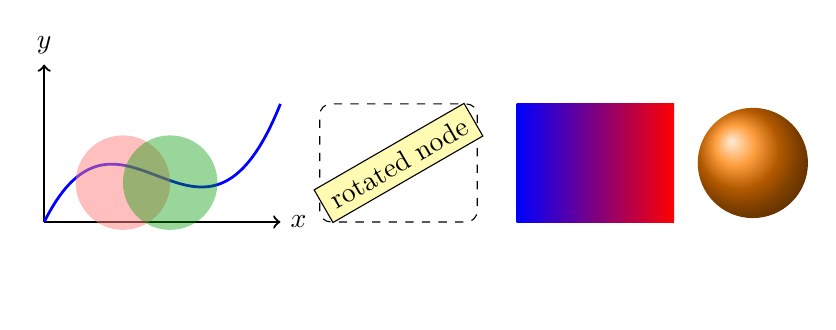
\begin{tikzpicture}
\draw[thick,->] (0,0) -- (3,0) node[right]{$x$};
\draw[thick,->] (0,0) -- (0,2) node[above]{$y$};
\draw[blue, line width=1pt] (0,0) .. controls (1,2) and (2,-1) .. (3,1.5);
\fill[red!50, opacity=0.5] (1,0.5) circle (0.6);
\fill[green!60!black, fill opacity=0.4] (1.6,0.5) circle (0.6);
\draw[dashed, rounded corners] (3.5,0) rectangle (5.5,1.5);
\node[draw, rotate=30, fill=yellow!30] at (4.5,0.75) {rotated node};
\shade[left color=blue, right color=red] (6,0) rectangle (8,1.5);
\shade[ball color=orange] (9,0.75) circle (0.7);
\end{tikzpicture}


\begin{tikzpicture}[scale=0.8]
\foreach \i in {0,...,11} { \draw[rotate=\i*30, color=purple!\the\numexpr\i*8\relax] (0,0) -- (2,0); }
\draw[draw opacity=0.3, line width=6pt] (3,0) -- (6,2);
\node[text opacity=0.5, font=\Large] at (4.5,0.5) {semi-transparent text};
\end{tikzpicture}
\end{document}
